\chapter{State of the Art}
\label{ch:State of the Art}
This chapter provides background on the various technologies used in the development of the proposed physical-digital system pair and describes the recent developments related to the Industry 4.0 features that have been provided in this system.
\section{Background Technologies}
\subsection{RIOT OS}
RIOT is a real-time operating system (OS) capable of multi-threaded operation, which supports a wide range of memory-constrained devices such as 8-bit and 16-bit microcontrollers and focuses on low-power wireless \acrshort{IoT} systems. It is an open-source OS and is well-documented \cite{Baccelli_RIOT_An_Open_2018}. It is based on a microkernel architecture and the software programming is generally implemented in C and C++. The microkernel architecture is well-suited for devices with restricted availability of non-volatile memory, as it provides nothing more than the minimum amount of software required for the functioning of the operating system. 

The kernel is hardware-independent and contains the basic functionality of the OS such as memory management and communication between various internal processes. The \acrshort{CPU} and board-specific configuration files are stored in separate directories, with corresponding sub-directories for each individual \acrshort{CPU} and board.

The RIOT architecture can be better described using Figure \ref{fig:structure}.
\begin{figure}
    \centering
    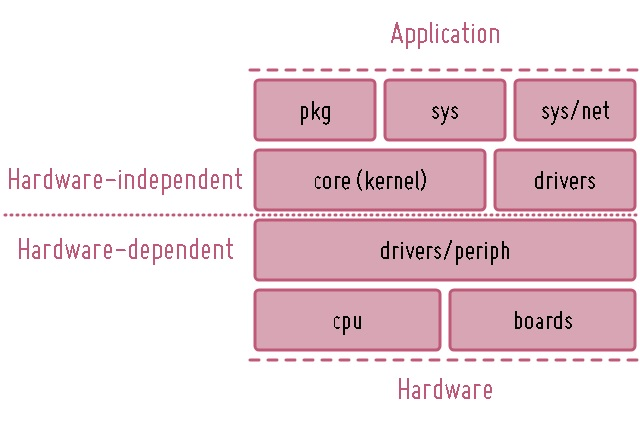
\includegraphics[scale=0.8]{images/RIOT_Structure.jpg}
    \caption{RIOT Structure \cite{Baccelli_RIOT_An_Open_2018}}
    \label{fig:structure}
\end{figure}

The applications built on RIOT OS for this thesis are compiled by GNU Make. It is typically used to compile source code into programs or libraries. The main element of the Make utility is the Makefile. The Makefile defines the rules and targets that Make uses to compile the specified source code. The action which is carried out by Make is called a recipe.

RIOT OS is a modular system, in which all features are implemented in separate entities, conveniently named as modules. These modules are built on top of the kernel and can be added individually in user applications. The modules are generally compiled using Make, but other compilers such as Valgrind are also supported.

There are several modules already developed and maintained by the RIOT community. Two such modules utilized in this thesis are SUIT, which provides functionality for Over-The-Air firmware updates, and GNRC Border Router, which can provide an interface between an IPv6 network such as the Internet and a mote device such as an \acrshort{MCU}. The SUIT module, combined with the GNRC border router, can be configured to update the device firmware over wireless interfaces such as \acrfull{BLE}, IEEE 802.15 or IEEE 802.11 (\acrshort{WiFi}).

\subsection{CoAP}
The \acrfull{CoAP} is a lightweight, machine-to-machine communication protocol, defined in RFC 7252 of the IETF \cite{rfc7252}. It was developed and standardized by the Constrained RESTful Environments (CoRE) Working Group of the IETF, and expanded by adding various new functions in order to make the protocol suitable for \acrshort{IoT} and M2M applications. It uses datagram-based transport protocol such as UDP, which makes it lightweight and desirable for low-power applications and networks such as 6LOWPAN.

\acrshort{CoAP} protocol is a client-server-based model that follows a request-response method, very similar to the widely used HTTP protocol. However, unlike HTTP, machine-to-machine interactions in \acrshort{CoAP} can lead to both machines taking up the role of a client and a server based on the use case. A \acrshort{CoAP} request is equivalent to that of HTTP and is sent by a client to request an action (using a Method Code) on a resource (identified by a URI) on a server.

Four message types are available in \acrshort{CoAP}: acknowledgment, reset, non-confirmable, and confirmable. This protocol includes message codes that identify the type of communication sent. \acrshort{CoAP} responses are typically accompanied by Acknowledgment messages, while \acrshort{CoAP} requests are typically sent as Confirmable or Non-confirmable messages. Safety-critical messages are transmitted using confirmable (CON) messages to guarantee dependability. They are sent with a message ID, and until the recipient sends an Acknowledgment message (ACK) with the same Message ID, they are retransmitted with a default timeout and exponential back-off between retransmissions. For non-critical communications, such a single reading from a continuous sensor data measurement, non-confirmable (NON) messages can be utilized.  NON messages do not carry an acknowledgment (ACK), but they do have a message ID that can be used to identify duplicates. Retransmission can be enabled by a recipient sending a Reset (RST) message in the event that it is unable to process a request message.

As shown in Figure \ref{fig:coap_format}, \acrshort{CoAP} can be rationally described as a two-layer protocol, with the message codes serving as the data layer and UDP serving as the asynchronous messaging layer. On the other hand, \acrshort{CoAP} is a single protocol that just includes the message and the Method or Response code in its message header.
\begin{figure}
    \centering
    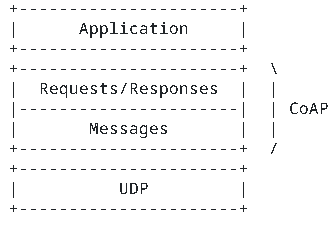
\includegraphics{images/CoAP Format.png}
    \caption{Abstract Layering of \acrshort{CoAP} Protocol \cite{rfc7252}}
    \label{fig:coap_format}
\end{figure}

\subsection{Over-The-Air Updates}
\acrfull{OTA} firmware updating is the process of providing wireless updates to the system of a terminal device, typically carried out over the internet. \acrshort{OTA} updates for the firmware of the microcontrollers allow for remote maintenance and secure operation of the MCU.

\acrshort{OTA} updates have become increasingly common in recent years, as they offer a convenient way for device manufacturers and developers to deliver new features and fix bugs without requiring users to physically connect their devices to a computer. This can be particularly useful for devices that are not easily accessible, such as those that are embedded in vehicles or other equipment.

\acrshort{OTA} updates are typically delivered in the form of a package that contains the update files and instructions for installing the update. The device's operating system or a dedicated update application is responsible for downloading and installing the update. Some \acrshort{OTA} updates may require the device to be restarted in order to complete the installation process.

There are several advantages to using \acrshort{OTA} updates \cite{nilsson2008_2}. For device manufacturers, they can reduce the cost of distributing updates, as they do not have to rely on physical media or require users to bring their devices to a service center. For users, \acrshort{OTA} updates can be more convenient, as they do not have to go through the process of connecting their device to a computer in order to receive the update. Additionally, \acrshort{OTA} updates can ensure that devices are kept up to date with the latest security patches and other important updates.

However, there are also some potential drawbacks to \acrshort{OTA} updates. If the update process is interrupted, it can result in a failed update, which may cause the device to become unstable or even inoperable. Additionally, some \acrshort{OTA} updates may require a significant amount of data to be downloaded, which can result in higher data usage and longer update duration.

Overall, \acrshort{OTA} updates offer a convenient and efficient way for device manufacturers and developers to deliver updates to their products and have become an important part of the modern device ecosystem.

\acrshort{SUIT}, short for \acrlong{SUIT}, is a firmware update infrastructure developed for RIOT OS by the IETF Working Group \cite{suit-23}. The \acrshort{SUIT} specification is a standard for securely delivering updates to \acrshort{IoT} devices, and it is designed to ensure that updates are authenticated, integrity-protected, and delivered in a manner that is resistant to attacks. It enables secure firmware updates for low-power \acrshort{IoT} devices using the \acrfull{CoAP}.

The \acrshort{SUIT} module in RIOT allows developers to build devices that are capable of securely receiving and installing updates \acrfull{OTA}, without the need for a physical connection to a computer. This can be particularly useful for \acrshort{IoT} devices, as it allows them to be updated remotely and without the need for user intervention.

The \acrshort{SUIT} module in RIOT is implemented using a combination of cryptographic techniques, such as digital signatures and hashing, to ensure the authenticity and integrity of updates. It also includes mechanisms to allow devices to verify the identity of the update server and to detect any tampering or modification of the update package.

The \acrshort{SUIT} module in the RIOT codebase resides in the sys/suit subdirectory in which the storage of the firmware image on the flash memory of the board and transport of the image file through \acrshort{CoAP} is implemented.

\subsection{Digital Twin}
A digital twin is a virtual replica of a physical system, designed to monitor the physical system using various sensors and interact with it using different communication protocols. The concept of a digital twin is a high-level construct, with many interpretations depending upon the area of application and the industry in question. As such, a digital twin can be anything from a simple block description of a process to a complex virtual simulation of an industry.

In the context of Industry 4.0, a digital twin can be used to monitor a manufacturing process by obtaining sensor data regarding various aspects of the process such as conveyor speed, position, occupation, and other such parameters. This data can then be relayed to the software model to run simulations or conduct various tests for performance improvements, all of which can then be used to manipulate the physical system to improve productivity.

There are multiple softwares available for out-of-the-box applications of a digital twin, that is, they can be installed and can be immediately put to use by creating virtual models of the physical modules and developing the required communication paths between them. After careful consideration of the available softwares and the required features, Unity3D has been selected for the purpose of developing a digital twin for this thesis.

One of the main features of Unity is its ability to import and work with assets from a variety of programs, such as 3D modeling software, audio editing software, and image editing software. This allows developers to easily incorporate a wide range of media into their projects. In addition to its asset import capabilities, Unity also has a robust set of tools for designing and building virtual environments, including a visual scripting system and a physics engine. These tools allow developers to create complex and interactive simulations. The 3D models for the factory modules used in this thesis have been designed in an open-source 3D modeling software called Blender, and the asset import feature of Unity has been used to incorporate these models in a simulation. The various object manipulation tools in Unity have allowed for motion simulation of the modules to reciprocate the motion of the physical system.

Unity also has a large and active community of developers, with a wealth of resources and support available online. This includes a comprehensive manual, tutorials, forums, and assets.

\subsection{Factory Planing Laboratory}
The Factory Planning Laboratory built by the Institute of Logistics and Material Handling at OVGU Magdeburg is a prototypical implementation of the logistics of a manufacturing unit \cite{lang}. The laboratory consists of factory module prototypes which can be used to simulate manufacturing paths and processes such as production, storage, and dispatch of a product. The modules that are available in the laboratory can be categorized into four types, which are, conveyors, turntables, sliders, and pushers.

Conveyors can be used for lateral movement in one dimension without any rotation. Turntables can provide rotation and provide lateral movement in one dimension. Sliders can provide two-dimensional lateral movement. Pushers can be used to ensure the proper path of the product or discard unnecessary products by pushing them into or out of the plane of the modules.

The modules in the Factory Planning Laboratory are designed by Fischertechnik \cite{fischertechnik_1965} and can be assembled manually from parts provided by them, which makes it easier to develop a modular factory model with several options for customization. Initially, Arduino Mega 2560 was used as the controller board for these modules in the laboratory, but for the purpose of network connectivity and multi-threading in this thesis, it was replaced by Nucleo F767ZI board.

\section{Related Work}
This section describes the current research in the literature regarding each individual facet of this thesis and then describes the current state of the art of the Digital-Physical system pair.

\subsection{\acrshort{OTA} Updates}
Updates for \acrshort{CPS} are relatively rare, especially when compared to personal computers or mobile devices. For example, in automotive systems, the frequency of updates is very low and mostly available only through dealerships. However, observations of recent trends suggest growth in automotive \acrshort{OTA} updates. 

Rapid advancement in \acrfull{IoT} technology gave rise to increased research on the methods and processes of Over-the-Air firmware updates for \acrshort{IoT} devices in the past few years. A few relevant systematic analyses are presented here for context. Firstly, an overview of the necessity of \acrshort{OTA} updates is presented. Then, some methods of \acrshort{OTA} updates are discussed and compared.

Bauwens et.al. presented an excellent approach to defining some key requirements of \acrshort{OTA} updates \cite{bauwens2020article}. In their study, an analysis is performed concerning the distribution of software development efforts in different parts of widely used \acrshort{IoT} operating systems. The software modules are divided into four blocks, applications, network, core OS and platform. Memory usage and Git commit history for each block are calculated for different \acrshort{IoT} operating systems. These calculations lead to the conclusion that application software for most \acrshort{IoT} systems occupies much less memory and requires much less update frequency when compared to the network protocol stack. It is calculated that 60\% to 84\% of the firmware updates are related to the network protocol stack. Hence, the authors have concluded that without network protocol updates, it is not possible to guarantee the optimal performance of an \acrshort{IoT} device during its operation lifetime.

After analyzing the need for \acrshort{OTA} updates, some \acrshort{OTA} update methods are presented here. In a journal article published by Halder et. al., research has been conducted on \acrshort{OTA} updates in the automotive industry, focusing mainly from a security perspective \cite{halder2020article}. They discuss the key security issues, challenges, and requirements necessary for \acrshort{OTA} updates and provide detailed background and comparison on various secure \acrshort{OTA} update techniques available in the current works of literature. Though the majority of this study focuses on the automotive sector, the update techniques described in the study provide a solid foundation for further analysis. Some of the techniques are summarized below.
\begin{itemize}
\renewcommand{\labelitemi}{$\bullet$}
    \item Symmetric Key Encryption: A set of link keys are shared between the Software Supplier, OEM, and the device. When a software update is needed, the Software Supplier uses a link key as a symmetric key with the device, encrypts the software, and sends it to the device for updation \cite{mahmud2005}.
    \item Hash Function: The binary file of the software to be updated is divided into multiple data fragments. Each fragment is encrypted using a pre-shared encryption key and transmitted to the device \cite{nilsson2008}.
    \item Blockchain: All devices participating in the update process are grouped into a cluster, with a designated cluster head. The cluster heads are connected in an overlay network to form a hierarchically connected system without a central controller. The Software Distributor triggers an update process by sending a store request to the cloud server. After receiving an acknowledgment from the cloud, the Software Distributor uploads the new software to the cloud, creates a transaction in a Blockchain block indicating the location of the latest software in the cloud, and broadcasts it to all the devices in the cluster\cite{steger2018-xo}.
    \item Hardware Security Module: A Hardware Security Module is used to store a cryptographic key and perform encryption during a software update. In this method, a gateway device downloads the software update from a remote server and validates it. If the validation is successful, it transfers the software to the target device. The advantage of using this technique is that it supports multiple encryption methods such as AES, RSA, SHA, etc. \cite{petri2016}. 
\end{itemize}

A novel method of \acrshort{OTA} update has been proposed by Guissouma et.al. where they proposed an approach covering the entire Software Development Life Cycle (SDLC) of an \acrshort{IoT} system \cite{Guissouma2020}. An important part of their work is their special attention given to variant and configuration management. Initially, three types of updates are defined
\begin{itemize}
\renewcommand{\labelitemi}{$\bullet$}
    \item Adaptive Updates: Updates that are performed to introduce new functionality into the system.
    \item Corrective Updates: Updates that are performed for error corrections and bug fixes.
    \item Perfective Updates: Updates that are performed for optimization of processes.
\end{itemize}
The method used is called a contract-based design, where a contract is a mathematical construct defined as a tuple \emph{C = (A,G)}. The assumption A stands for a condition on the environment of a component M and the guarantee G describes a property that the component guarantees to satisfy if A holds. The \acrshort{OTA} update process is triggered by the violation of a contract. 

\subsection{Digital Twin}
Current developments of digital twins in the industry have been described by Tao et al.\cite{tao2019}. They reviewed the most relevant theories in their paper, which can be divided into four parts as Modeling, simulation, verification, validation, and accreditation (VV\&A); data fusion; interaction and collaboration; and service. They have further summarised the industrial applications of Digital Twins, as being used majorly in Product Lifecycle, for patents and applications by industry leaders.

The dimensions of digital twin applications have been summarised by Enders and Hoßbach\cite{enders2019}. They described six dimensions which are the industrial sector, purpose, physical reference object, completeness, creation time, and connection. In their paper, they stated that the manufacturing industry is one of the major fields where digital twins are applied, and the three main purposes of the digital twin are stated as simulation, monitoring, and control. These dimensions are the cornerstone for the implementation of the digital twin in this thesis.

Vijayakumar et al. developed a Digital Twin for factory system simulation in \cite{vijayakumar2019digital}. The aim of this work is to develop a new methodology for reducing the amount of time and cost of keeping the manufacturing facility updated. They have used Plant Simulation for the development of the simulation model and Autodesk Navisworks for the visualization of the factory. The results are promising, with a 96.6\% reduction in the monitoring process. However, this system is unidirectional, in essence, only uses the Digital Twin to monitor the system, but does not provide a firmware update feature.

Wahab et al. \cite{wahab2023} proposed a project to design and develop an AR Aid as an alternative learning tool training guidance for the operational setup of an electrical discharge machine. The key feature of their work is the use of Unity software to develop the Digital Twin and Blender software to develop the animations, both of which are used in this thesis,

\subsection{Factory Planning Laboratory}
The Factory Planning Laboratory at OVGU Magdeburg has already been utilized for experimentation of various factory environment simulations over the course of two years. Initially, the storage of products in a storage matrix is simulated in \cite{Sankaramanchi_I-4_0-learning-Laboratory-_2023}, where a High-Bay Shelf was assembled and utilized for experimentation. Later, a complete factory layout with separate production, storage, and dispatch zones was developed to provide proof of concept for different wireless communication methods between the factory modules. Different wireless communication protocols such as \acrshort{LiFi}, Bluetooth, UART, and RF are implemented to demonstrate inter-protocol connectivity and modularity of the system. \cite{Sankaramanchi_I-4_0-learning-Laboratory-_2023}

\subsection{Digital-Physical System Pair}
Grznár et al. \cite{grznar2020modeling} discussed the future of manufacturing systems with regard to technological innovation and factory planning. They described that digitization and the application of exponential technologies are extremely important to CPS. The manufacturing systems in the future will be designed as modular, reconfigurable and independent systems. To keep up with such a system, it is absolutely essential to develop a Digital Twin in constant communication with the physical system, which is termed here as a Digital-Physical System Pair.

Within the context of manufacturing, there have not been many instances of a combination of a digital twin with \acrshort{OTA} firmware updates in the literature. The closest resemblance to the work proposed in this thesis is conducted in the BASE MoVE research project by J. Akelbein et al \cite{mci/Akelbein2021}. This project provides a modular base platform for \acrshort{IoT} applications. A proof-of-concept is provided by implementing the platform on a home automation system.

The BASE MoVE project used RIOT OS for its modularity, debug support, and support of an open compiler to create a sensor node hardware platform with support for \acrshort{OTA} updates using the SUIT module.

This project has also been equipped with multiprotocol support, where IPv6 protocols such as 6LoWPAN and \acrshort{BLE} are included. The native 6LoWPAN stack in RIOT OS was utilized. \acrshort{BLE}, which is included in different smart home products and almost all smartphones, was implemented using the open-source stack called nimBLE which is currently integrated into RIOT OS. Additionally, the Thread protocol was also included in this group, where they used the OpenThread implementation due to its portability to RIOT OS. The IP transport protocol that was used in this project is the \acrfull{CoAP}, as it is relatively lightweight and uses UDP. Initially, they used the \acrshort{CoAP} implementation from RIOT OS to manually map the sensor data provided by their devices to a REST structure. Some limitations such as compatibility and interoperability led to the development of a second approach using a prototypical implementation of a subset of Dotdot, which is a universal language of \acrshort{IoT} to enable devices to work together on a network. Due to limitations of documentation and the unavailability of open-source specifications, this implementation was only restricted to sensor polling over \acrshort{CoAP} and 6LoWPAN.

The platform was evaluated by developing a home automation system, where a house was retrofitted. The sensors were attached to the windows and doors to provide data of the state, either open or closed. Two scenarios S1 and S2, respectively named Ambient Assisted Living scenario and Smart Home scenario were evaluated within multiple rooms, using various protocols mentioned before.

Finally, J. Akelbein et al concluded that their approach for an IoT solution is feasible. They reported that RIOT OS has served their purpose well, with clear signs of improvements in the future. After careful consideration of the conclusions provided in their paper, the use of OpenThread protocol for this thesis was rejected as they reported memory leaks and energy consumption issues. However, their documentation on wireless implementation is not satisfactory. Although they mentioned the use of \acrshort{BLE} initially, they did not include it in their final evaluation due to a lack of support. There was also no consideration of a WiFi-based implementation, although the present generation of home automation systems almost always includes WiFi.

To summarize, the necessary background of the different technologies used in this thesis is provided and recent developments in those technologies are outlined. In light of the described works and their drawbacks, this thesis aims to accommodate the features that proved to be proper additions to a factory layout and omit the remaining features. The following chapter provides a conceptual model of the proposed work and details the implementation of the factory layout.